\section{Appendix/ Evaluation}
\label{sec:appx-evaluation}
% Evaluation write-up built from BubbleTea-results/eval (figures + CSVs in eval/); every number traces to a
% CSV in eval/ (named in the comment above each figure). Labels carry an appx- prefix so they don't clash
% with sections/evaluation.tex.
\acresetall

We evaluate \sys{} on three \ac{MoE} models and ask four questions.
First, how much fine-tuning throughput does \sys{} extract while serving
keeps its latency, compared with an iteration-level colocation system and
with plain colocation (\S\ref{sec:appx-eval-e2e})? Second, which of \sys{}'s
mechanisms is responsible for the gain (\S\ref{sec:appx-eval-mech})? Third, does
\sys{} still help once the serving engine balances expert load itself
(\S\ref{sec:appx-eval-eplb})? Fourth, what does \sys{} cost when it has nothing
to do, in serving latency and in GPU memory, and does it train correctly
(\S\ref{sec:appx-eval-overheads})?

%-------------------------------------------------------------------------------
\subsection{Methodology}
\label{sec:appx-eval-method}

\paragraph{Hardware and software.}
All experiments run on one node with four NVIDIA A100-SXM4-80GB GPUs connected
by NVLink (NV12 between every pair). Serving uses vLLM with \ac{TP}$=$\ac{EP}$=4$
unless stated otherwise, bf16 weights, eager execution, chunked prefill and
prefix caching disabled, and a 0.85 GPU-memory budget.
\sys{} runs its trainer as a separate process per GPU under CUDA MPS, as
described in \S\ref{sec:design}, with a 50\,$\mu$s chunk budget and a
60\,$\mu$s early-close margin.

\paragraph{Models.}
Qwen3-30B-A3B (48 layers, 128 experts, top-8), Qwen1.5-MoE-A2.7B (24 layers,
60 routed experts, top-4) and DeepSeek-V2-Lite (27 layers, 64 routed experts,
top-6). Qwen1.5-MoE's configuration declares an 8k context; for longer prompts
we size its rotary cache to the served length, for every system alike.

\paragraph{Serving workload.}
Requests are arXiv summarization prompts cut to an exact length of
1k--32k tokens, each producing 32 output tokens. Each run sends 400 requests
at a constant arrival rate. For every prompt length we pick three rates:
\emph{high} is just below the point where vLLM alone starts to queue, and
\emph{medium} and \emph{low} are fixed fractions of it per model. We also
replay two production traces (\S\ref{sec:appx-eval-traces}). Latency statistics
exclude the first and last 10\% of each run's requests and pool the
requests of all repetitions; throughput is averaged over repetitions.
Every cell runs twice (vLLM + torchtune once).

\paragraph{Fine-tuning workload.}
Every system trains the same job: LoRA rank 16 on the attention
projections ($q,k,v,o$; for DeepSeek-V2-Lite $q$, $kv_a$, $kv_b$, $o$), on
alpaca-cleaned samples padded to 128 tokens, with AdamW at learning rate
$2\cdot10^{-4}$. We report fine-tuning throughput as samples per second
completed while requests are being served.

\paragraph{Systems.}
\begin{itemize}
  \item \textbf{vLLM alone} is the serving reference; all latency ratios are
    relative to it, measured in the same campaign on the same node.
  \item \textbf{vLLM + torchtune} is off-the-shelf colocation: a stock
    torchtune LoRA recipe (FSDP over the four GPUs, its own copy of the model)
    runs next to vLLM under MPS with no coordination. We cap the trainer at
    6\% of each GPU's \acp{SM} (MPS active-thread percentage); without the
    cap it disrupts serving far more (\S\ref{sec:appx-eval-e2e}).
    vLLM's memory budget is lowered to 0.70 to make room for it.
  \item \textbf{LLMStation}~\cite{llmstation} is the state of the art in
    iteration-level colocation: it trains inside the serving engine between
    and alongside serving iterations. We port it to the same three models; its
    latency ratios are taken against its own engine with training switched
    off, so that differences between the two engines do not count against
    either system.
  \item \textbf{\sys{}} is the full system: decode/idle-time colocation
    plus intra-layer bubble harvesting, two training chains with adaptive
    pairing, device-side exchanges and early close.
\end{itemize}

%-------------------------------------------------------------------------------
\subsection{Fine-tuning throughput at serving latency}
\label{sec:appx-eval-e2e}

% Data: eval/fig62_*.csv (BubbleTea-results/eval/s62/v4: collect_v4.py -> s62.json, make_figs.py).

\begin{figure*}[t]
  \centering
  \includegraphics[width=\textwidth]{eval/fig62_1_ft_throughput.png}
  \caption{\textbf{Fine-tuning throughput while serving.} Samples per second
    for \sys{}, LLMStation and vLLM + torchtune across prompt lengths and
    three load levels per model; labels give \sys{}'s throughput relative to
    LLMStation.}
  \label{fig:appx-eval-e2e-tput}
\end{figure*}

\begin{figure*}[t]
  \centering
  \includegraphics[width=\textwidth]{eval/fig62_2_p90_ttft.png}\\
  \includegraphics[width=\textwidth]{eval/fig62_2_p90_tpot.png}
  \caption{\textbf{Serving latency under colocation.} p90 \ac{TTFT} (top)
    and p90 \ac{TPOT} (bottom) for the cells of
    Figure~\ref{fig:appx-eval-e2e-tput}, relative to serving alone.}
  \label{fig:appx-eval-e2e-lat}
\end{figure*}

\paragraph{Throughput.}
Figure~\ref{fig:appx-eval-e2e-tput} shows the headline result. Across all three
models, seven prompt lengths from 1k to 32k tokens and three loads (63
cells), \sys{} trains 1.9--6.2$\times$ faster than LLMStation, 2.8$\times$
in the median cell. The gap is widest exactly where LLMStation struggles: at
high load. On Qwen3-30B-A3B with 4k prompts at
8 requests/s, LLMStation finds only 0.20 samples/s of room because the
engine is rarely idle and the decode iterations are short, while \sys{} still
trains 1.00 sample/s, almost all inside prefill bubbles that iteration-level
scheduling cannot see. At low load both systems mostly train in idle
time, and \sys{}'s advantage (1.9--3.1$\times$) comes from executing the
compiled step efficiently rather than from bubbles.

\paragraph{Latency.}
Figure~\ref{fig:appx-eval-e2e-lat} shows what this costs. In 50 of the 63
cells, \sys{} keeps both p90 \ac{TTFT} and p90 \ac{TPOT} within 10\% of
serving alone, and in the median cell it adds 4\% to \ac{TTFT} and 6\% to
\ac{TPOT}. That is the property the admission window is built for: the
most-loaded GPU, which sits on the critical path, almost never admits
training, and every other GPU stops admitting a margin before its bubble
ends. LLMStation, measured against its own engine alone, stays within the band
in 44 of the 63 cells, so the throughput gap above is not bought with
latency.

Most of the cells outside the band share one cause: decode latency on
Qwen1.5-MoE with long prompts. At high load p90 \ac{TPOT} rises by
1.20$\times$ at 16k, 1.38$\times$ at 24k and 1.30$\times$ at 32k, and the
effect is there at lower loads too (1.14--1.47$\times$ from 16k up).
Qwen1.5-MoE's decode steps are short (about 30\,ms), and with long prompts
the engine spends most of its time in prefill, so the decode iterations that
remain carry the trainer's cross-GPU exchanges. Replacing the exchanges with
no-ops brings decode steps back to vLLM's (at the cost of wrong gradients, so
only as a diagnostic), which identifies the exchanges, not the bubble
harvesting, as the cause. The other two models, with longer decode steps,
do not show the effect.

\paragraph{Short prompts.}
At 1k and 2k tokens a single prefill is too short to be worth harvesting
(\sys{} only opens windows in forward passes of at least 4k prefill tokens),
so most of its training runs in decode and idle time, as LLMStation's does.
\sys{} still trains 2.5--3.6$\times$ faster at low and medium load, and
2.9--6.2$\times$ faster at high load, where LLMStation's iteration-level
slack all but disappears. Latency stays within the 10\% band in 15 of the
18 short-prompt cells, and a sixteenth (Qwen3-30B-A3B, 2k, low load) misses
it by a point. The other two are at the highest request rates we
run, 16 requests/s of 1k prompts on Qwen3-30B-A3B and 32 requests/s on
Qwen1.5-MoE. In the first, p90 \ac{TTFT} rises by 1.13$\times$. In the
second, the trainer's decode-time work is enough to tip the engine into
queueing, and p90 \ac{TTFT} reaches 3.6$\times$ that of vLLM alone (0.63\,s
against 0.18\,s). LLMStation queues even more in the same cell, at
1.24\,s. At such request rates there is little time left in which training
can run without delaying someone.

\paragraph{Off-the-shelf colocation.}
The simplest alternative to both systems is to run an ordinary trainer next
to vLLM and let the GPU share itself. Capped at 6\% of the \acp{SM},
vLLM + torchtune is a reasonable serving neighbour: it keeps both p90
\ac{TTFT} and p90 \ac{TPOT} within the 10\% band in 51 of 63 cells. But it
trains only 0.2--1.3 samples/s, a median 5.9$\times$ slower than \sys{}
(6.5$\times$ in the cells where it holds the band). Nine of its twelve
misses are at high load, the worst on DeepSeek-V2-Lite with 1k prompts at
16 requests/s, where its p90 \ac{TTFT} is 9.4$\times$ that of vLLM alone.
It trains faster than \sys{} in a single cell, DeepSeek-V2-Lite at 8k and
7 requests/s (0.80 against 0.65 samples/s), and pays for it with
6.2$\times$ vLLM's p90 \ac{TTFT}. Among the cells where both systems stay in
the band, the closest it comes is DeepSeek-V2-Lite at 4k and 12 requests/s,
where \sys{} trains 1.14$\times$ faster. Removing the cap does not help:
the uncapped trainer is only 1.2$\times$ faster in the median cell, holds the
band in just 6 of 63 cells, and pushes p90 \ac{TTFT} up to 31$\times$ that of
vLLM alone. Without coordination, a trainer either takes the GPU while
requests wait or is throttled until it barely trains.

\paragraph{Smaller parallel groups.}
% Data: eval/fig62_4_tp2.csv (BubbleTea-results/eval/s62/v4/make_tp2.py over grid_eplb/tp2).
\begin{figure*}[t]
  \centering
  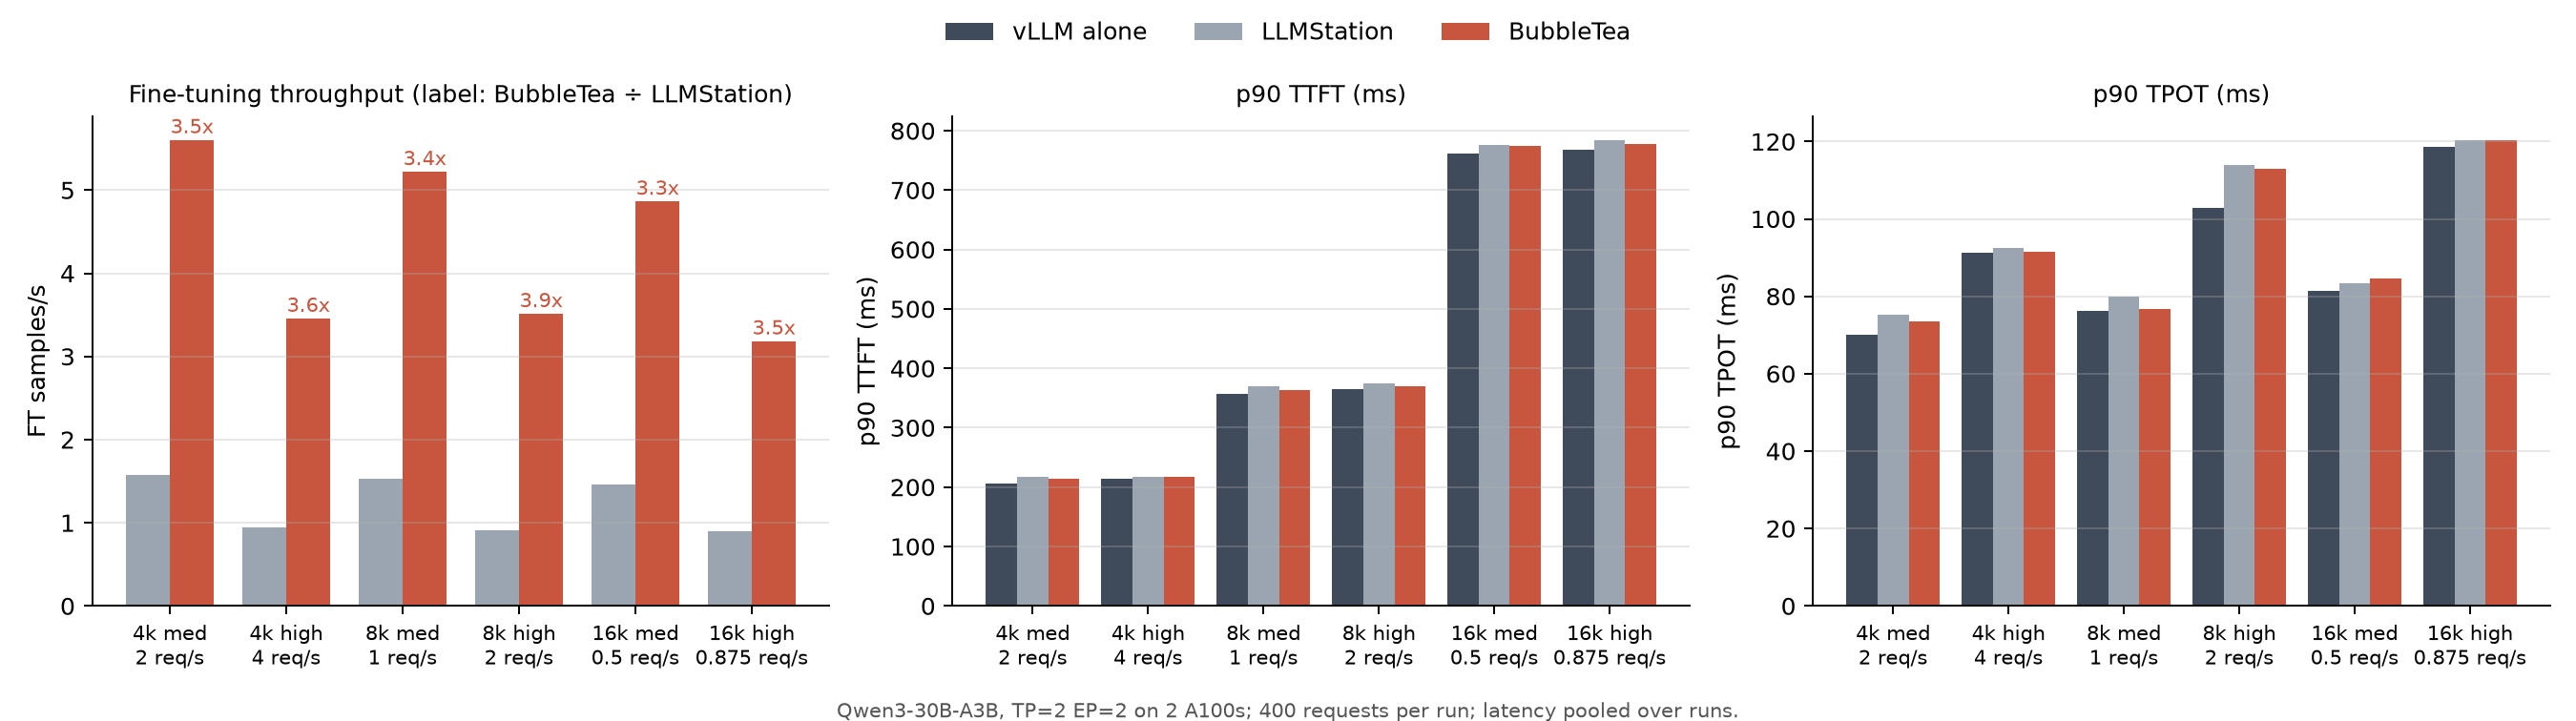
\includegraphics[width=\textwidth]{eval/fig62_4_tp2.png}
  \caption{\textbf{Qwen3-30B-A3B at \ac{TP}$=$\ac{EP}$=2$} on two A100s.
    Left: fine-tuning throughput (labels: \sys{} relative to LLMStation).
    Middle and right: p90 \ac{TTFT} and \ac{TPOT} of all three systems.}
  \label{fig:appx-eval-tp2}
\end{figure*}
Nothing in \sys{} assumes four GPUs. Figure~\ref{fig:appx-eval-tp2} serves
Qwen3-30B-A3B on two GPUs (\ac{TP}$=$\ac{EP}$=2$, each GPU holding 64
experts) with 4k, 8k and 16k prompts at medium and high load, where high is
again the highest rate at which vLLM alone does not queue at this size.
\sys{} trains 3.3--3.9$\times$ faster than LLMStation here, every cell
above the four-GPU median of 2.8$\times$. At high load LLMStation trains
under one sample per second in every cell, while \sys{} still trains
3.2--3.5 samples/s. Both systems keep p90 latency close to serving alone:
\sys{} stays within 10\% of vLLM in every cell (the largest increase is
p90 \ac{TPOT} at 8k and high load, 1.10$\times$), and LLMStation within 11\%.

\paragraph{Traces.}
\label{sec:appx-eval-traces}
\begin{figure}[t]
  \centering
  \includegraphics[width=\columnwidth]{eval/fig62_3_trace.png}
  \caption{\textbf{Production traces} (Qwen3-30B-A3B). Top: request
    arrivals. Bottom: fine-tuning throughput and p90 latency.}
  \label{fig:appx-eval-traces}
\end{figure}
Fixed-length, evenly spaced requests are the easiest case for any scheduler.
Figure~\ref{fig:appx-eval-traces} replays ten minutes of two Azure LLM inference
traces at their original rate: the code trace (long prompts, very short
outputs) and the conversation trace (shorter prompts, longer outputs), both
with bursty arrivals. \sys{} trains 5.9 and 5.0 samples/s against
LLMStation's 1.8 and 1.5, a 3.2$\times$ advantage, while p90 \ac{TTFT}
and \ac{TPOT} stay within 7\% of serving alone on both traces.
vLLM + torchtune (6\% cap) also stays within 9\% of serving alone, but
trains only 0.37 samples/s on either trace, 13--16$\times$ less than \sys{}. Bursts do not
break the admission window: when a burst arrives the engine is in prefill,
which is precisely when bubbles appear.

%-------------------------------------------------------------------------------
\subsection{Where the throughput comes from}
\label{sec:appx-eval-mech}

\begin{figure*}[t]
  \centering
  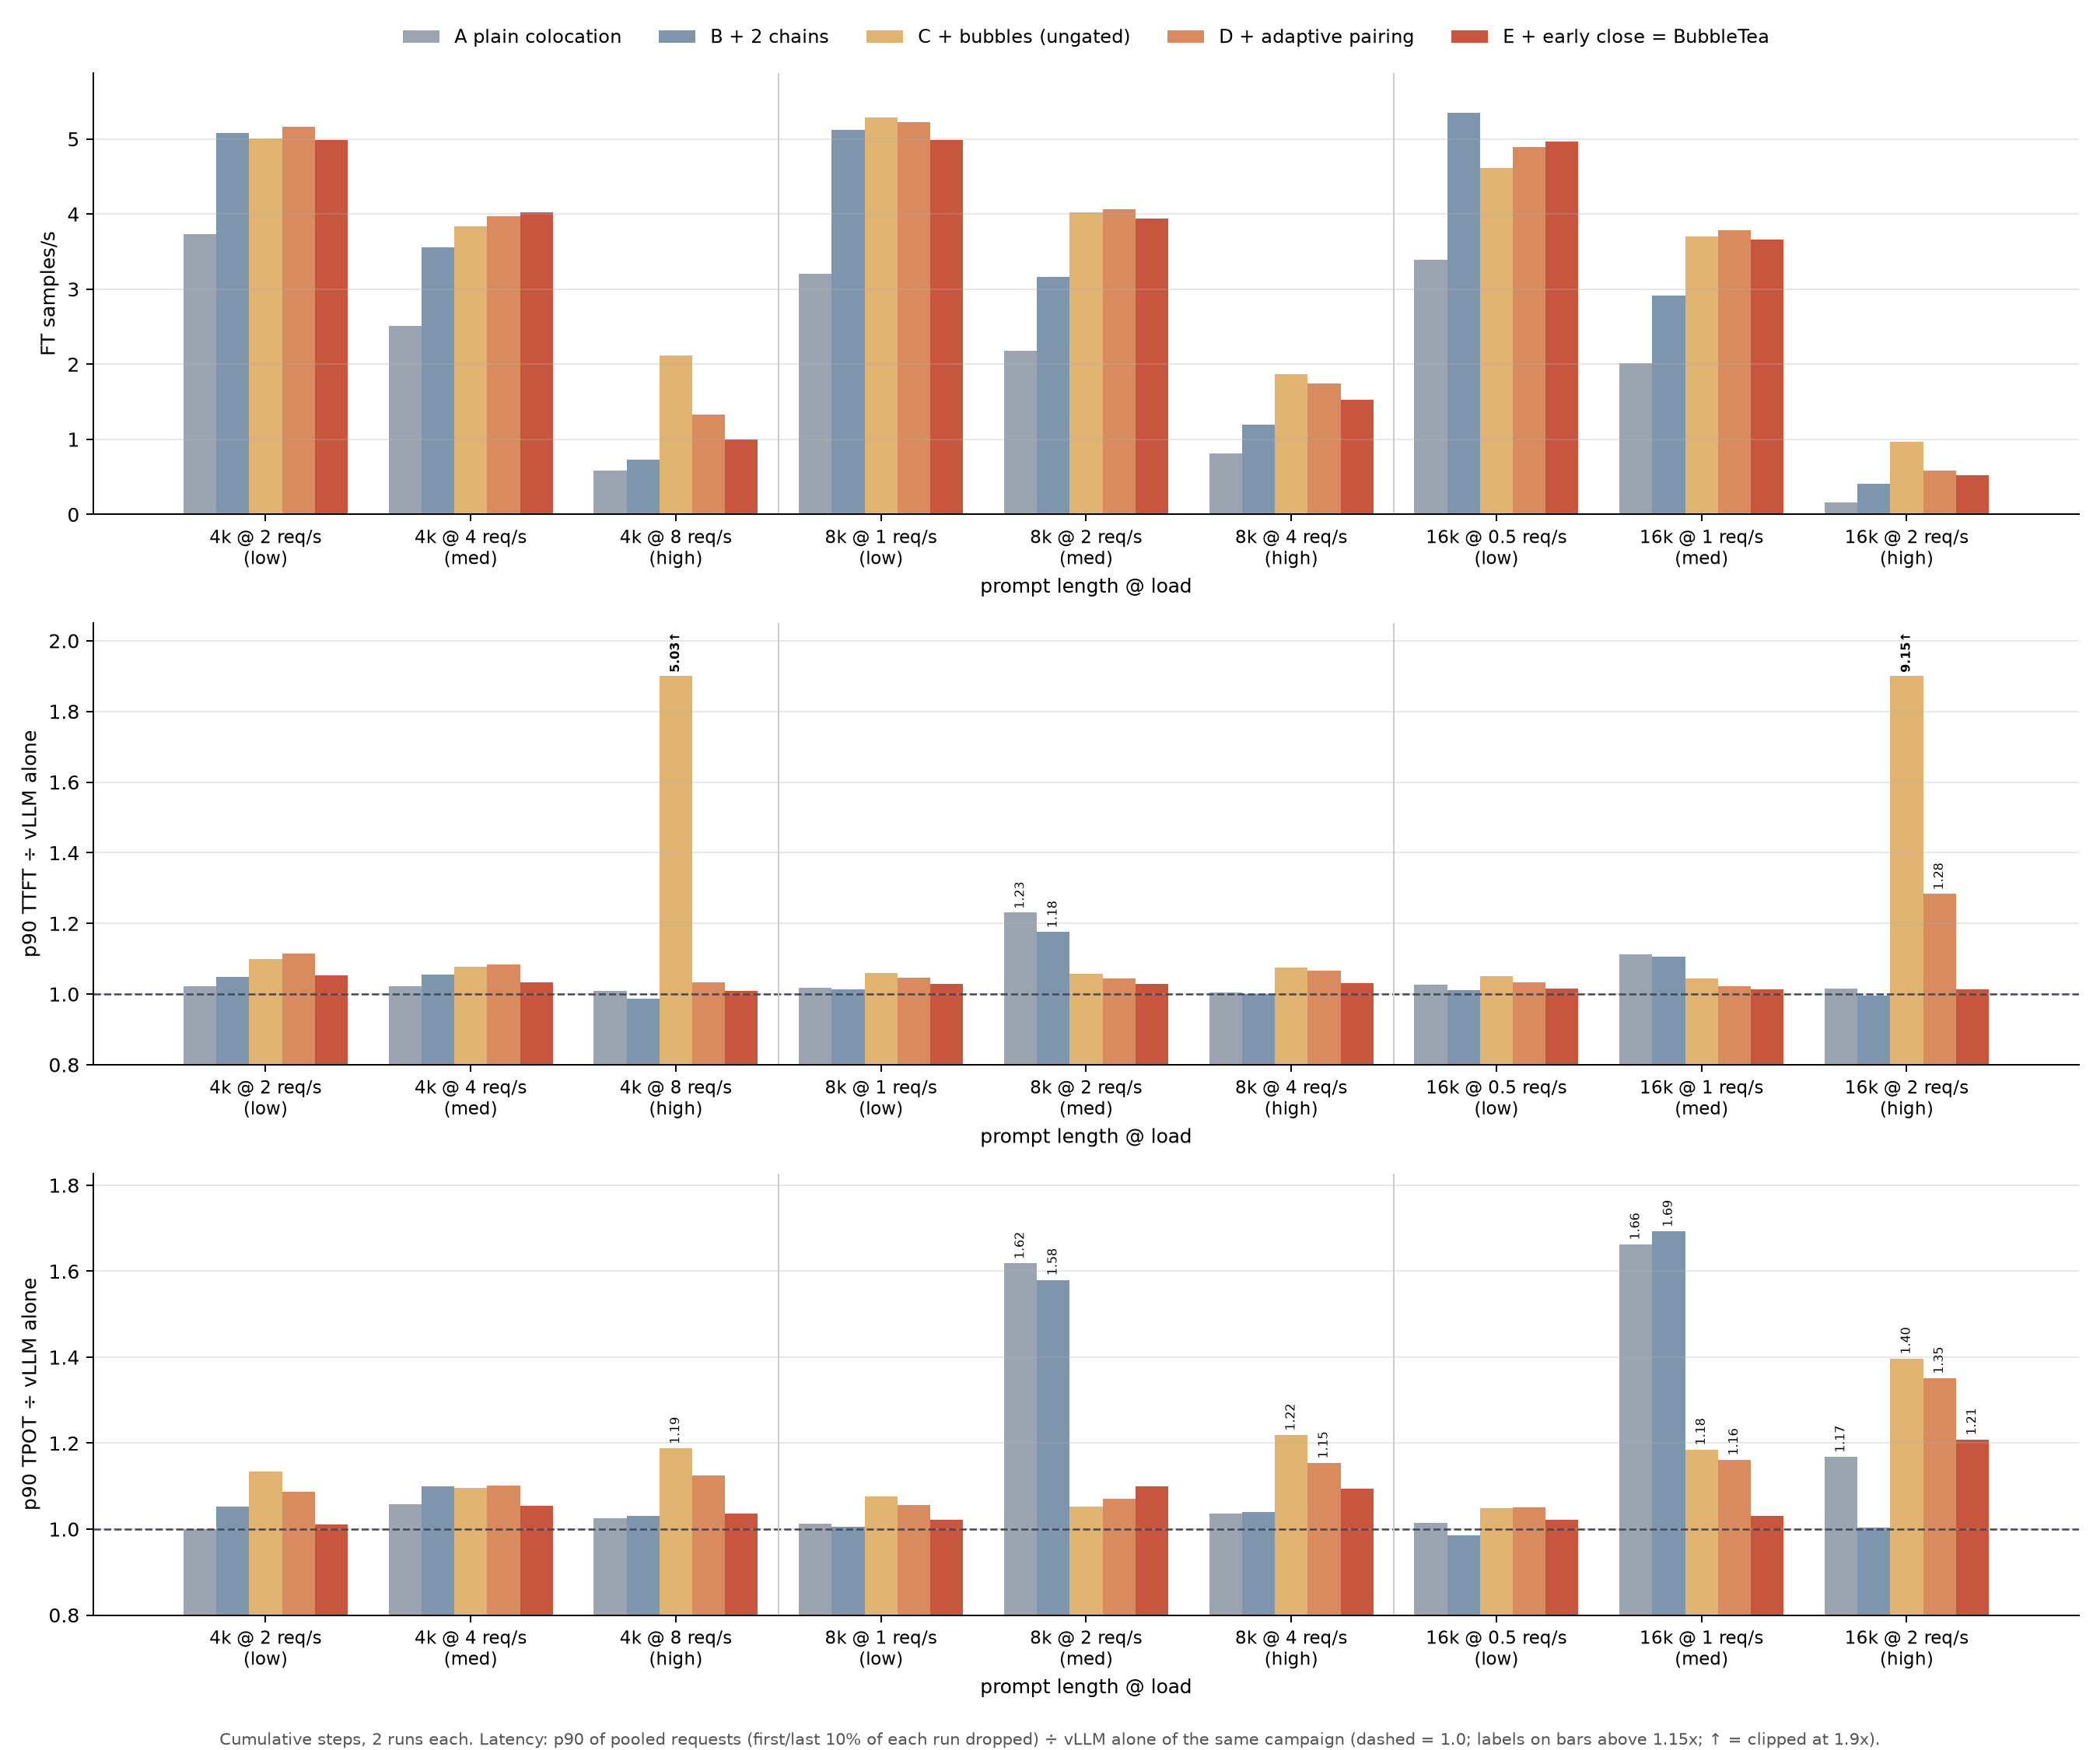
\includegraphics[width=\textwidth]{eval/fig63_ladder.png}
  \caption{\textbf{Mechanism ladder} on Qwen3-30B-A3B. Each step adds one
    mechanism to the previous one: (A) plain colocation in decode and idle
    time, (B) a second training chain with device-side exchanges, (C)
    training inside prefill bubbles with an always-open gate, (D) adaptive
    pairing of the two chains, (E) early close, i.e.\ \sys{}.}
  \label{fig:appx-eval-ladder}
\end{figure*}

Figure~\ref{fig:appx-eval-ladder} builds \sys{} up one mechanism at a time on
Qwen3-30B-A3B, across three prompt lengths and three loads.

Plain colocation (A) already trains 3.2--3.7 samples/s at low load, but at
high load it collapses to 0.16--0.82 samples/s because idle time
disappears. A second chain with device-side exchanges (B) keeps work
ready across exchange waits and adds 35--60\% at low and medium load.

Opening the prefill bubbles (C) is the step that changes the high-load
picture: throughput at high load rises 1.6--2.9$\times$ over (B). But an
always-open gate also admits training on the slowest GPU, and the latency
cost shows it: p90 \ac{TTFT} jumps to 5.0$\times$ at 4k and 9.2$\times$ at
16k at high load. Adaptive pairing (D) runs the second chain only when
it has useful ready work, which removes most of the queueing (p90 \ac{TTFT}
1.03$\times$ and 1.28$\times$) at a cost in throughput. Early close (E)
removes the rest: by closing each window a margin before the predicted end
of its bubble, and never opening one on the most-loaded GPU, \sys{} brings
p90 \ac{TTFT} to within 5\% of serving alone in all nine cells while keeping
most of the bubble throughput (0.5--1.5 samples/s at high load, against
0.4--1.2 for B).

The lesson matches \S\ref{sec:gap}: bubbles are worth harvesting only if
admission is decided per GPU and per layer. Bubbles alone (C) are fast and
unusable; with the predictor and early close they are both.

%-------------------------------------------------------------------------------
\subsection{Composition with expert load balancing}
\label{sec:appx-eval-eplb}

\begin{figure*}[t]
  \centering
  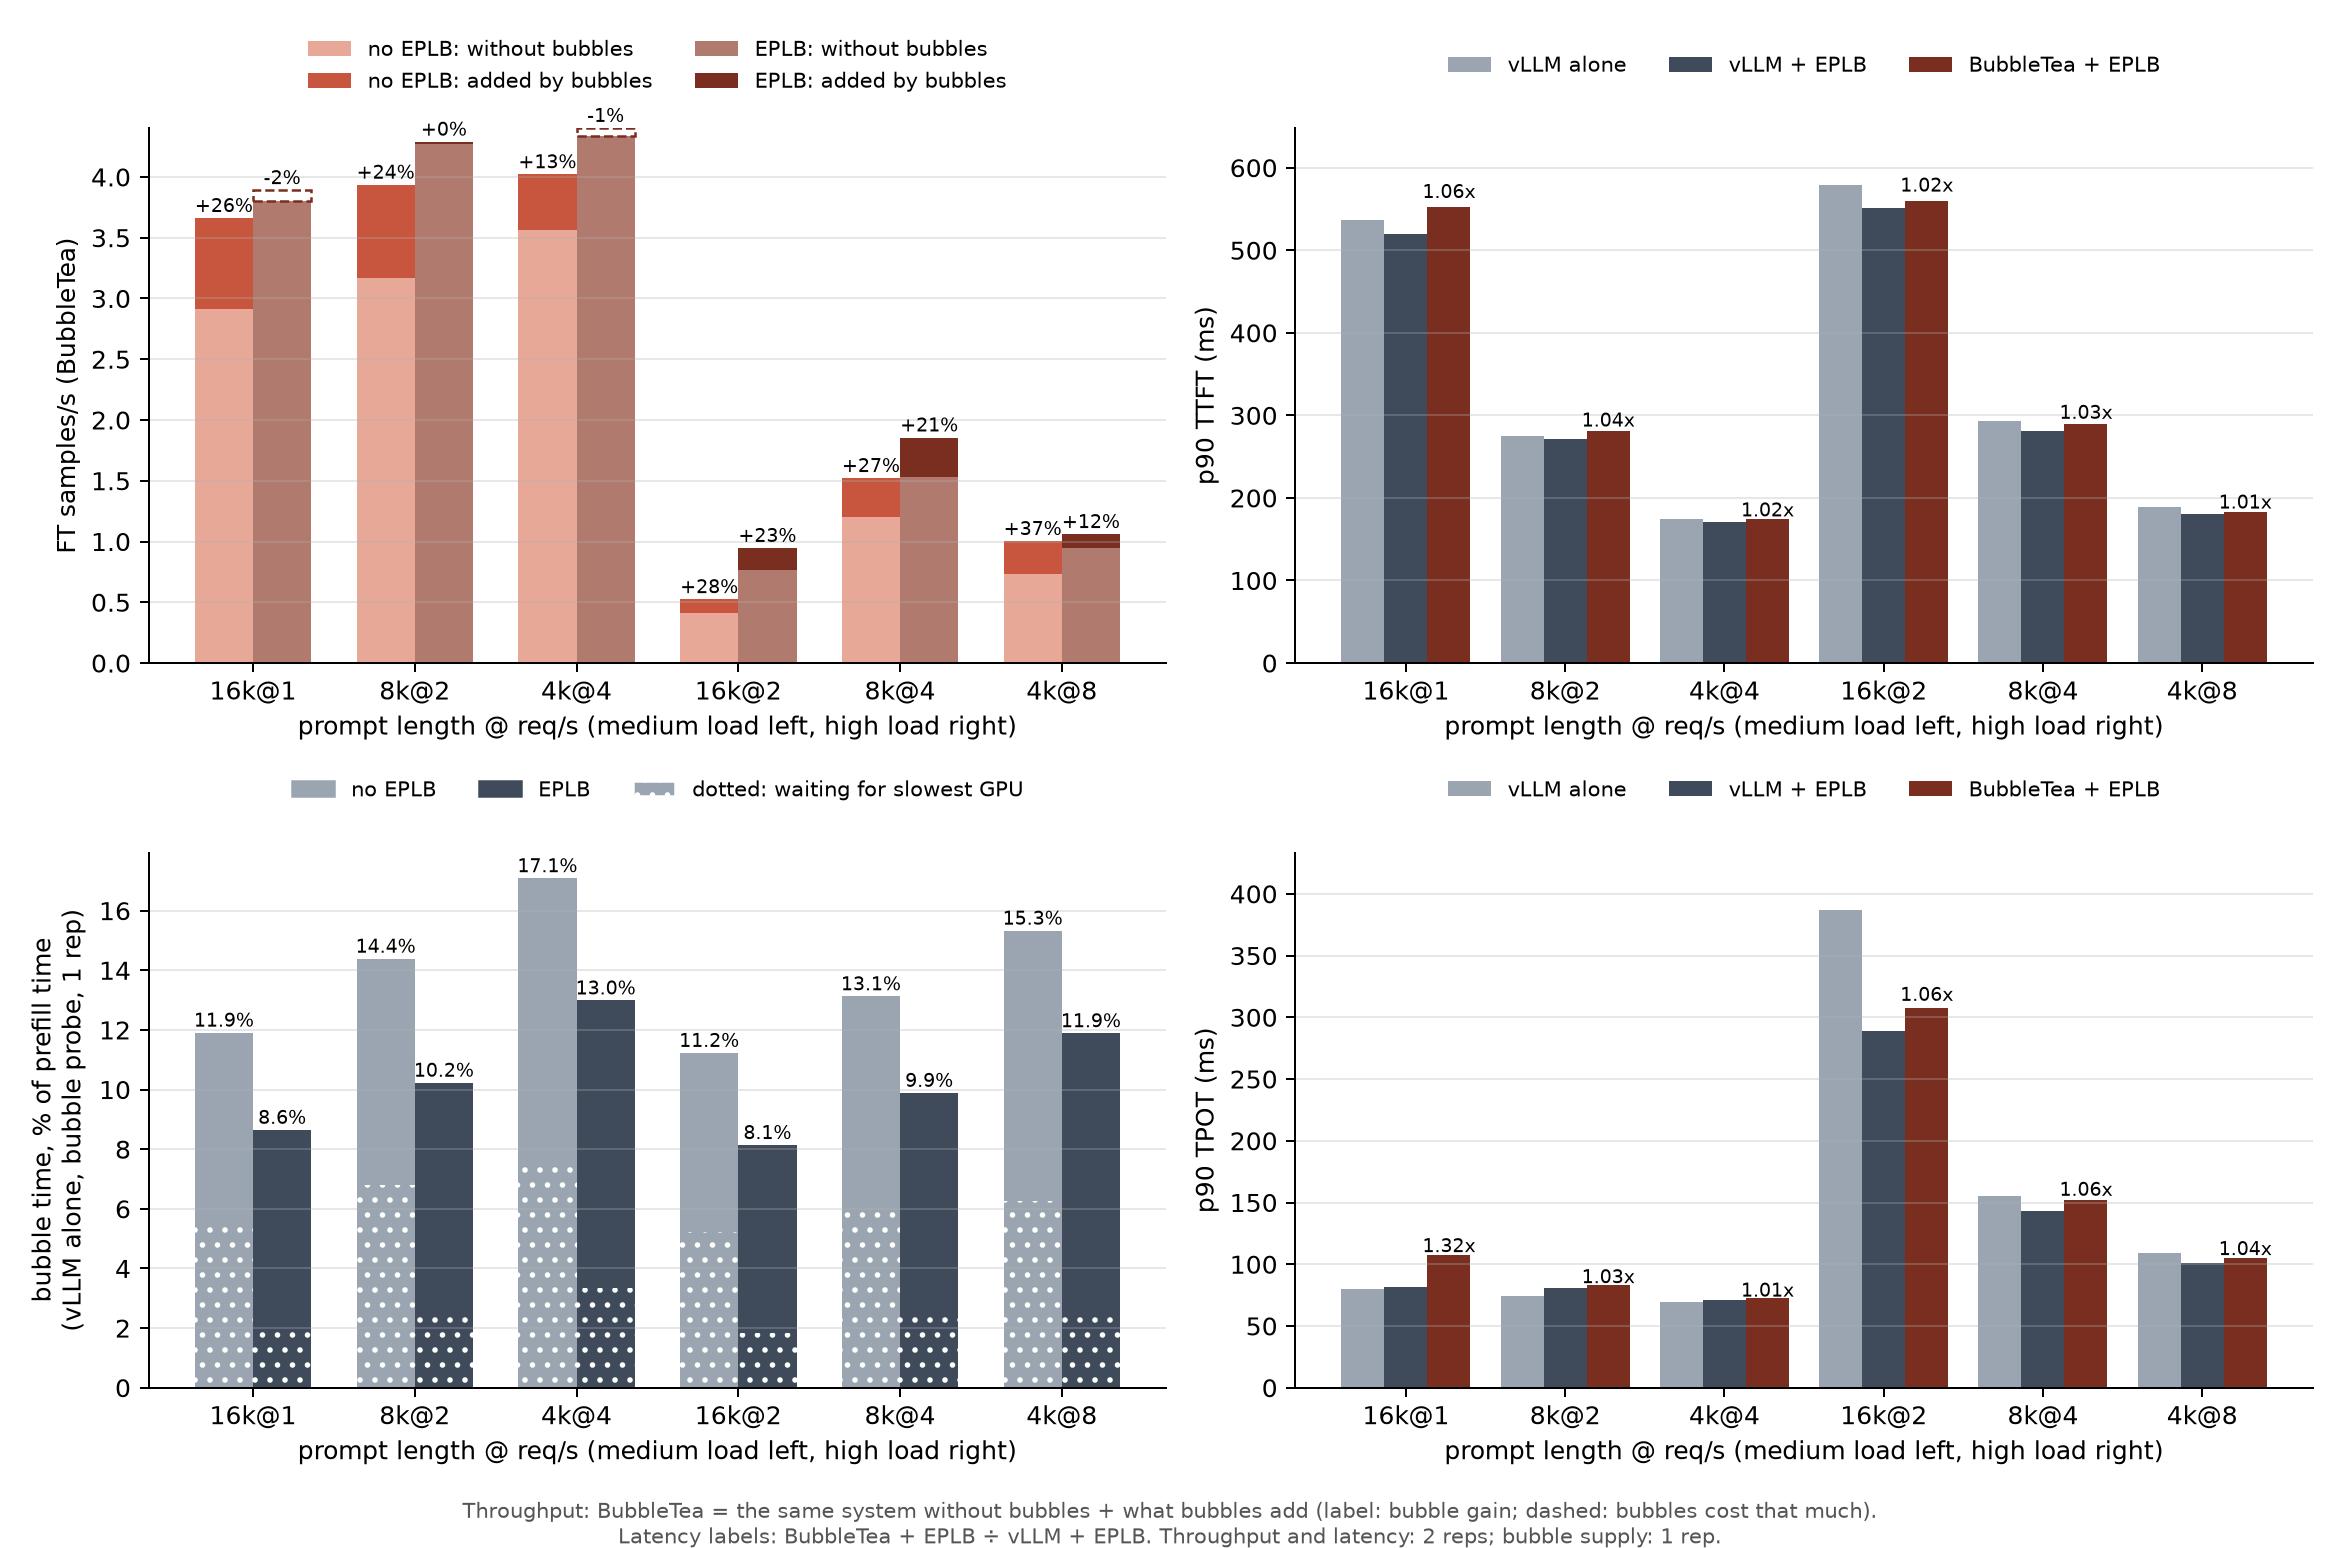
\includegraphics[width=\textwidth]{eval/fig64_eplb.png}
  \caption{\textbf{\sys{} with EPLB} (Qwen3-30B-A3B, 16 redundant experts).
    Bubble share of prefill time with and without EPLB, fine-tuning
    throughput with and without bubble harvesting, and latency relative to
    vLLM with EPLB.}
  \label{fig:appx-eval-eplb}
\end{figure*}

Load balancing attacks the same imbalance that creates bubbles, so the
natural question is whether \sys{} still pays off once the serving engine
balances its experts. We enable vLLM's EPLB with 16 redundant experts and
compare \sys{} with and without bubble harvesting
(Figure~\ref{fig:appx-eval-eplb}).

EPLB does what it promises: the bubble share of prefill time drops from
11--17\% to 8--13\%. It also helps colocation in general, because balanced
experts make the serving iterations themselves shorter; training without
bubbles gains 24--87\% from EPLB alone.

On top of EPLB, bubble harvesting still adds 12--23\% at high load, where
idle time is scarce and bubbles are the main source of slack. At medium load
it adds nothing measurable ($-2$\% to $+0$\%): with EPLB the idle-time
trainer already finds enough room, and the smaller residual bubbles do not
add to it. Latency with EPLB stays within 6\% of vLLM with EPLB, with one
exception: p90 \ac{TPOT} at 16k and 1 request/s is 1.32$\times$.

So EPLB and \sys{} compose: balancing should run first, and \sys{} picks up
the residual bubbles, which matter most when the system is busy.

%-------------------------------------------------------------------------------
\subsection{Bubble supply and use}
\label{sec:appx-eval-bubbles}

% Data: BubbleTea-results/eval/s65 (bubble probe, Oct 6-7, segments on, 1 rep; use breakdown from the Sep 30
% build, bt_8k2.txt, where segment graphs did not hide individual training kernels from the probe).
\begin{figure*}[t]
  \centering
  \includegraphics[width=\textwidth]{eval/fig65_bubble_supply.png}
  \caption{\textbf{Bubble supply} (Qwen3-30B-A3B). Left: share of prefill time
    spent in bubbles with vLLM alone, with and without EPLB; the dotted part is
    time spent waiting for the slowest GPU. Middle: bubble length (median, p90).
    Right: total bubble time at 8k and 4 requests/s when each configuration
    runs alongside, relative to vLLM alone.}
  \label{fig:appx-eval-supply}
\end{figure*}

How much is there to harvest, and how much of it does \sys{} use?
Figure~\ref{fig:appx-eval-supply} measures the supply with vLLM alone. Bubbles
take 11--17\% of prefill time on Qwen3-30B-A3B, and EPLB lowers that to
8--13\%. Individual bubbles are short: the median is 0.3--1.0\,ms and shrinks
with shorter prompts, because a layer's expert work is smaller. This is
the regime \S\ref{sec:gap} predicted, and it is why \sys{} works in
50\,$\mu$s chunks.

Training must not create bubbles of its own. The right panel shows the
total bubble time when each configuration runs next to serving. Plain
colocation leaves it unchanged, and an ungated trainer that also trains in
bubbles adds 17\%: it slows the most-loaded GPU, and every other GPU then
waits longer. \sys{} adds 4\% (2\% with a single chain), because the most
loaded GPU almost never opens a window.

On the use side, we account for every microsecond of bubble on the GPUs
that are not the straggler, at 8k and 2 requests/s. \sys{} trains during
36\% of that time. Another 50\% passes with the window open but no chunk
running---the trainer is waiting on its own cross-GPU exchange or has no
ready work---and 15\% is given up by closing early. Closing early is cheap
insurance: windows close before the slowest GPU arrives in 98\% of cases, a
median 57\,$\mu$s early, and the gate opens on the straggler in only 4\%
of layers. No training ran on serving's critical path outside a window. The
remaining open-but-idle time is the headroom for future work: a third chain
or finer-grained exchanges could fill part of it.

% Data: eval/fig_capacity.csv (BubbleTea-results/eval/s62/capacity/make_capacity.py over grid_*/capacity, vLLM
% alone with step + bubble probes, 2026-10-16/17; decode co-run microbenchmark in capacity/decode_corun).
\begin{figure*}[t]
  \centering
  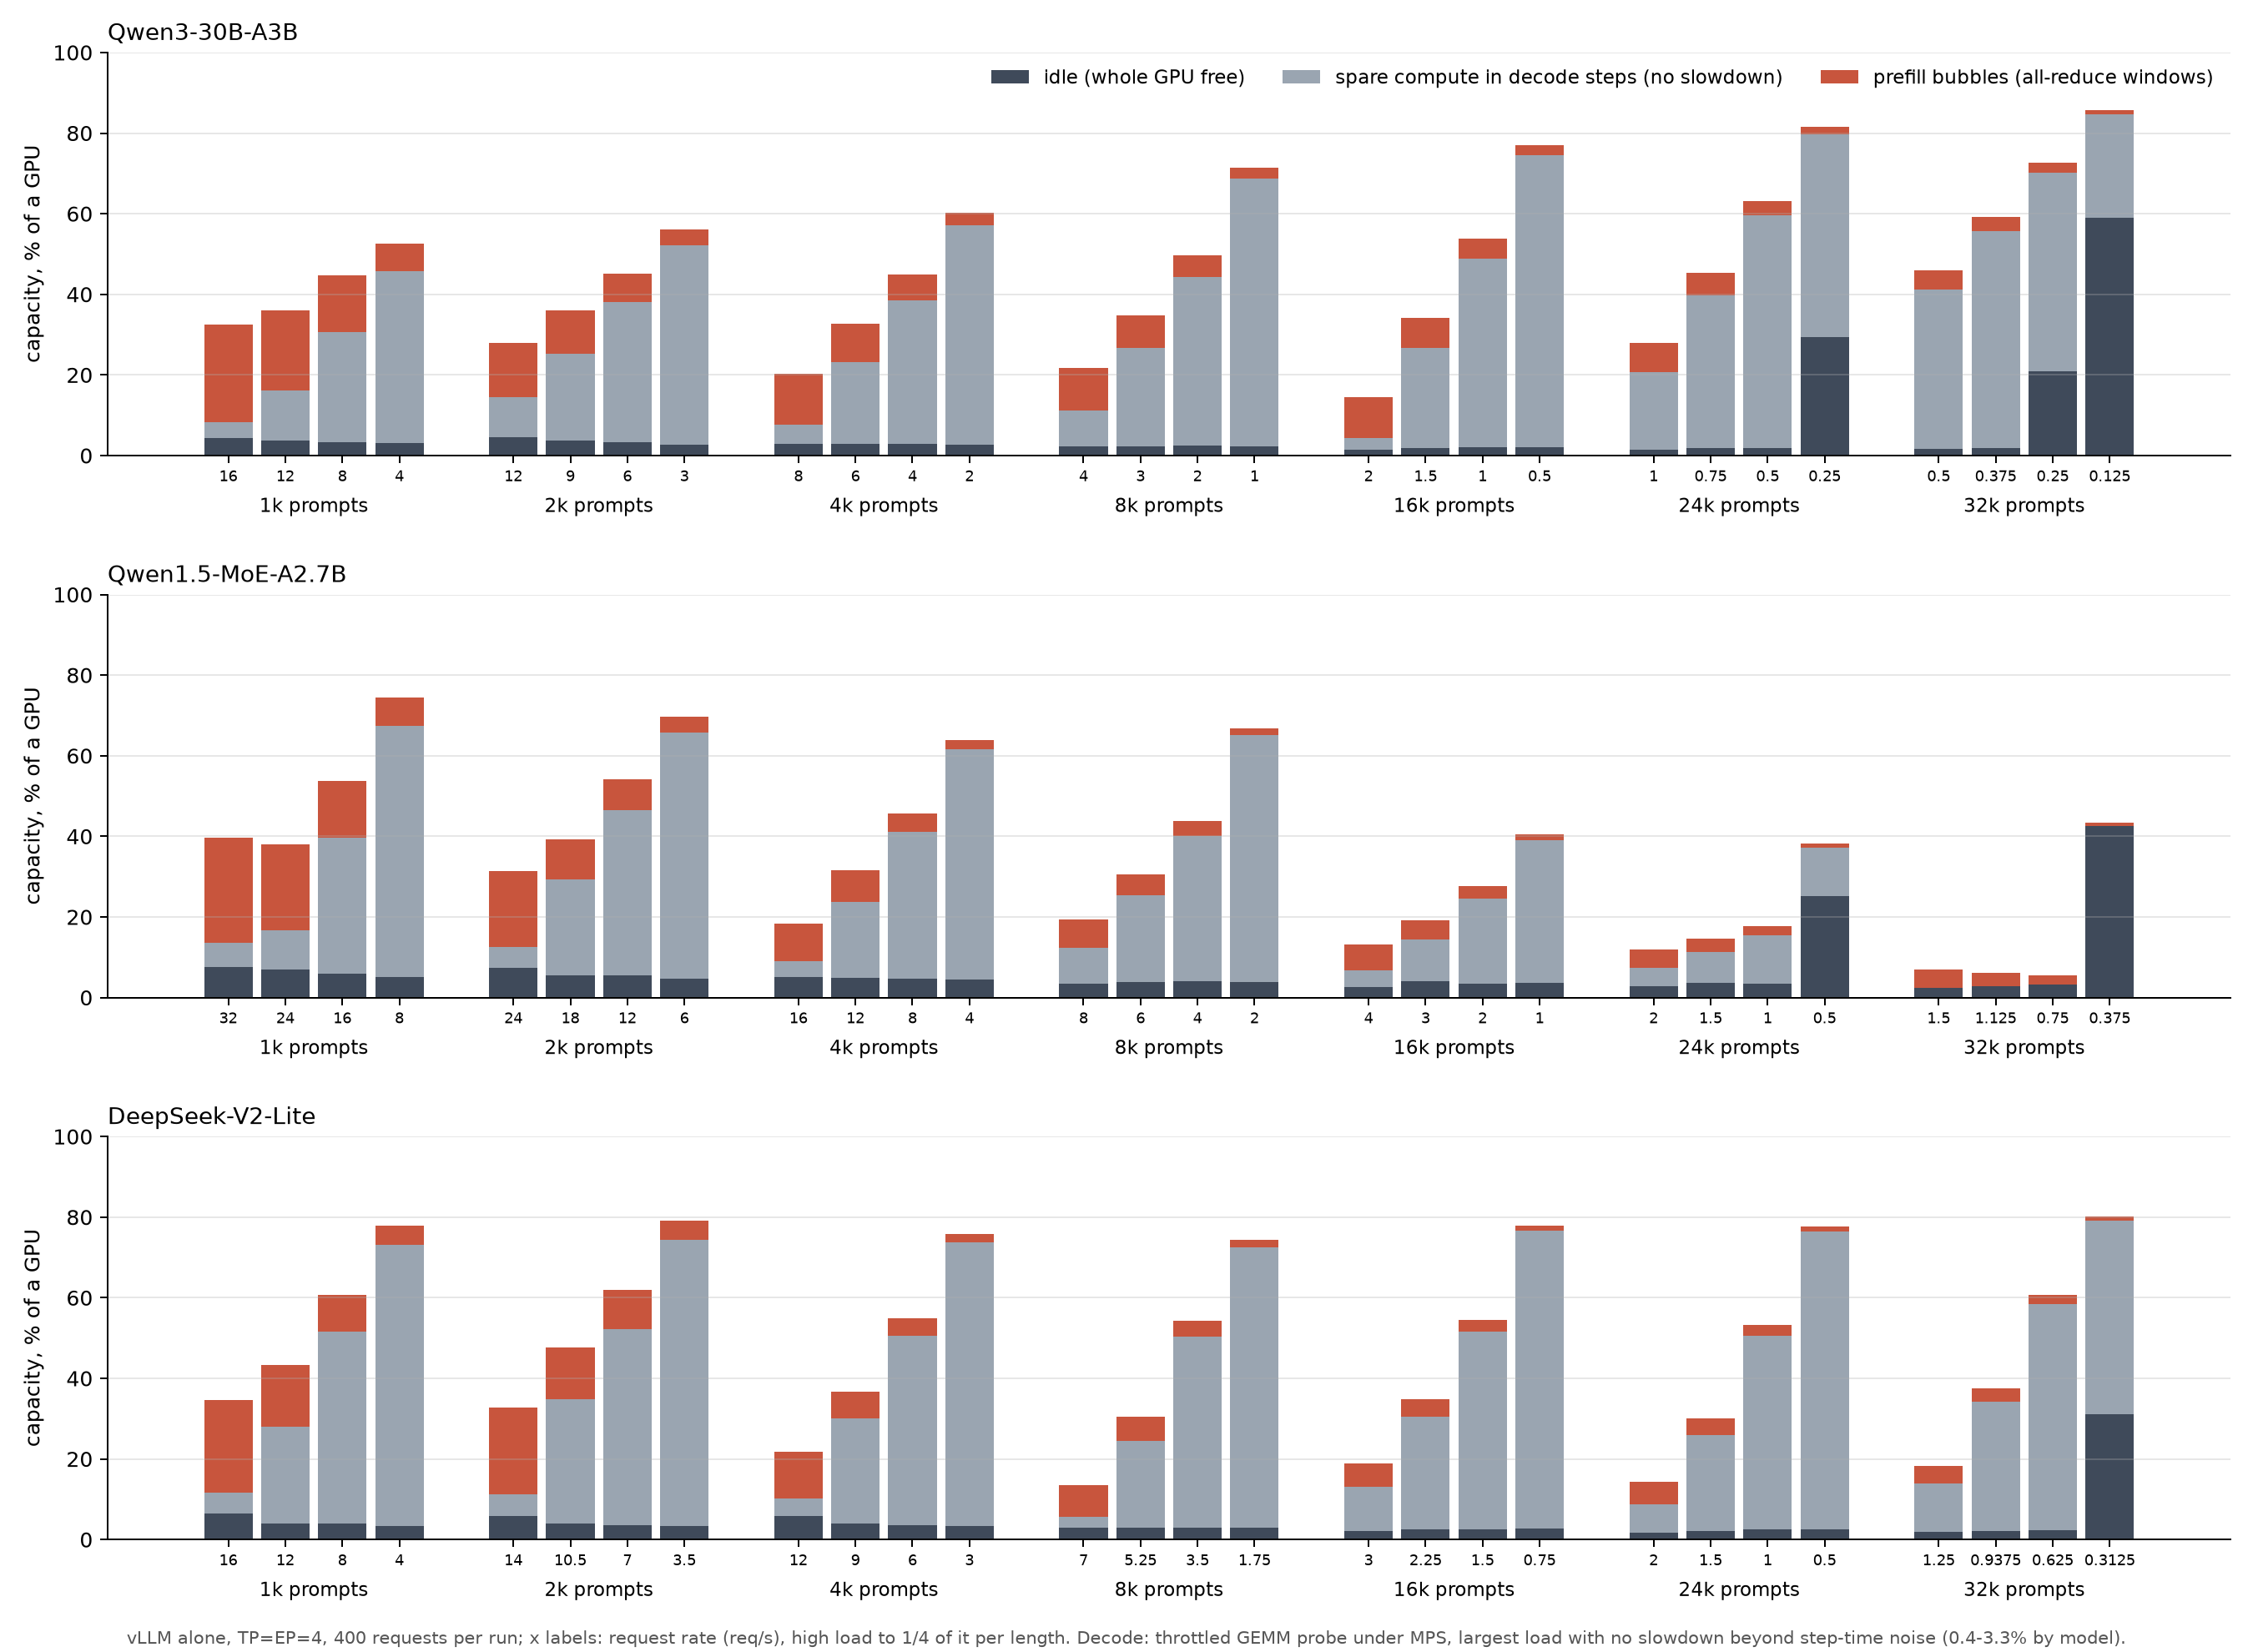
\includegraphics[width=\textwidth]{eval/fig_capacity.png}
  \caption{\textbf{Where the spare capacity is} (vLLM alone, 400 requests per
    run, high load down to a quarter of it). Idle: no forward pass running.
    Decode: the share of a free GPU's GEMM throughput a co-running job gets
    inside decode steps without slowing them beyond measurement noise.
    Bubbles: all-reduce windows of prefill MoE layers. All in percent of one
    GPU over the run.}
  \label{fig:appx-eval-capacity}
\end{figure*}

\paragraph{Where the spare capacity is.}
Bubbles are one of three places a co-located job can run. The other two are
idle time and the unused part of decode steps. Figure~\ref{fig:appx-eval-capacity}
measures all three with vLLM alone, across lengths and loads. For
decode, a throttled GEMM job runs next to fixed batches of decode requests,
and we keep the largest size that does not lengthen decode steps beyond
measurement noise (0.4--3.3\% depending on the model).

Decode steps are roomy. In eager mode they are bound by kernel launches
(30--55\,ms whatever the batch), and a co-running job gets most of the
GPU's GEMM rate inside them (47--98\%) without slowing them. At a quarter of the high
load, that makes decode the largest source by far: 35--74\% of a GPU up to
16k prompts. But it shrinks as load rises, because prefill takes over the
timeline: at high load it is down to 3--11\% from 1k to 16k prompts.

Bubbles behave differently. For a given model and prompt length they are a
fixed share of prefill time, whatever the load (within about two points
from 4k up), and that share falls with prompt length: from 20--31\% at 1k
to 6--9\% at 32k. So bubble capacity grows with load instead of shrinking,
and at high load it overtakes decode: in 13 of the 15 high-load cells from
1k to 16k, and in 7 of the 9 from 4k (where \sys{} harvests) to 16k.
Truly idle time is small (1--8\%) except at the lowest loads with 24k and
32k prompts (21--59\%).

This is the division of labour \sys{} relies on: iteration-level schemes
like LLMStation's can use decode and idle time, which is plentiful at low
load and scarce at high load; bubbles are the part of the timeline that
grows with load. Two caveats. These numbers are supply, not what \sys{}
harvests; the use measurement above puts that at about a third of the
bubble time.
And Qwen1.5-MoE at 32k is an outlier: even the smallest co-running job
slows its decode steps by 19--30\%, so there it has no decode capacity at
all (its 16k and 24k decode values are interpolated between the 8k and 32k
measurements).

%-------------------------------------------------------------------------------
\subsection{Overheads and correctness}
\label{sec:appx-eval-overheads}

\sys{} puts code on serving's critical path and keeps a trainer resident on
every GPU. This section measures what that costs when there is nothing to
gain, and checks that the model it trains is the model a normal trainer
would produce.

% Data: eval/fig66_sched_overhead.csv (make_sched2.py), eval/fig66_hook_cost.csv (hook_cost/microbench3.py).
\begin{figure*}[t]
  \centering
  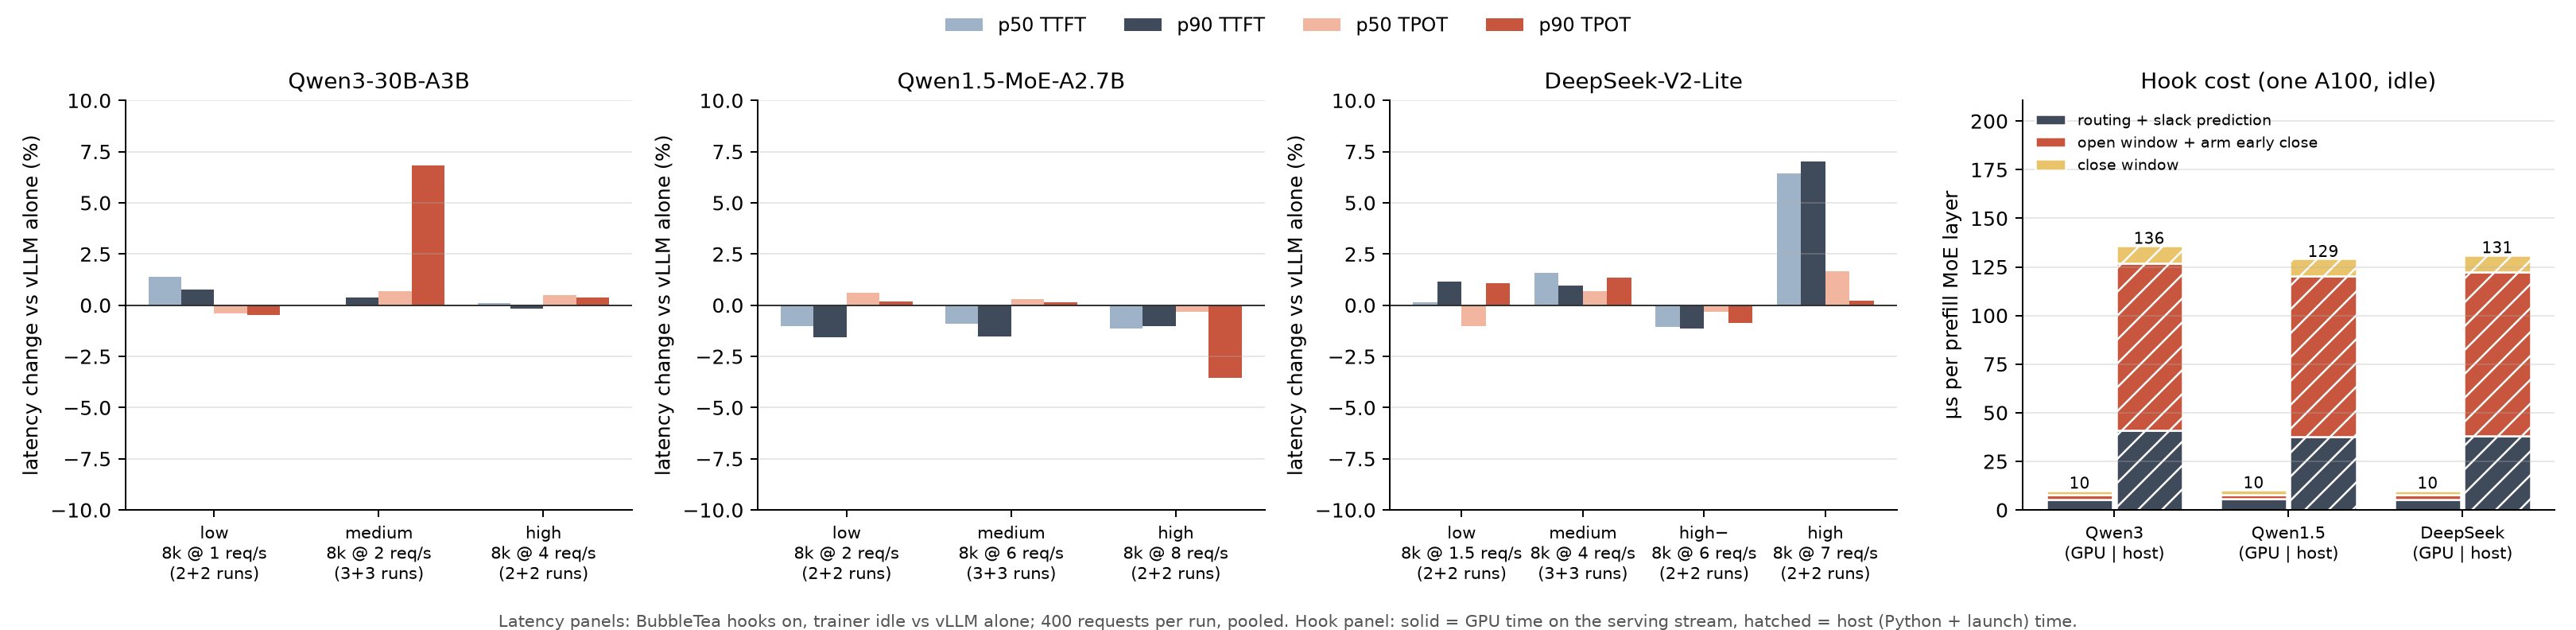
\includegraphics[width=\textwidth]{eval/fig66_sched_overhead.png}
  \caption{\textbf{Cost of the scheduling hooks.} Left three panels: latency
    with \sys{}'s hooks active and its trainer present but never admitted,
    relative to vLLM alone, with 8k prompts at three loads (2--3 runs of 400
    requests each per bar). Right: cost of the hooks for one prefill \ac{MoE}
    layer, on the GPU and on the host.}
  \label{fig:appx-eval-sched}
\end{figure*}

\paragraph{Scheduling.}
To isolate the scheduler, we run \sys{} with its trainer started but never
allowed to train. Every prefill \ac{MoE} layer still predicts its bubble,
opens a window, arms early close and closes it again, so serving pays for
all of the scheduling but gets nothing in return.
Figure~\ref{fig:appx-eval-sched} shows that this is cheap. On the GPU the three
hooks together take about 10\,$\mu$s per layer, against layer times of
several milliseconds for an 8k prefill. On the host they take
130\,$\mu$s per layer, or 3--7\,ms per forward pass, but that time overlaps
GPU execution: the measured duration of prefill steps does not change by
more than 0.5\% on any model.

Serving latency agrees. Across the three models and three loads, p50 and
p90 \ac{TTFT} and \ac{TPOT} stay within 2.5\% of vLLM alone in almost every
case, in both directions, which is the run-to-run noise of this setup. Two
points stand out. Qwen3-30B-A3B shows one 7\% increase in p90 \ac{TPOT} at
medium load that does not recur at the neighbouring loads. DeepSeek-V2-Lite
at its high load of 7 requests/s shows a consistent 6--7\% increase in
\ac{TTFT}, in both repetitions. That load keeps prefill busy 95\% of the
time, against 81--85\% for the other two models' high loads, and at that
utilization any added delay, even the sub-percent one above, compounds in the
prefill queue. At 6 requests/s (82\% utilization) the difference disappears
($-1$\%). In short, the hooks cost nothing measurable unless the server is
already at the edge of queueing.

% Data: eval/fig66_overheads.csv (make_overheads.py), eval/fig66_mem_breakdown.csv (make_membreak.py,
% mem_breakdown/analyze.py over allocator snapshots).
\begin{figure*}[t]
  \centering
  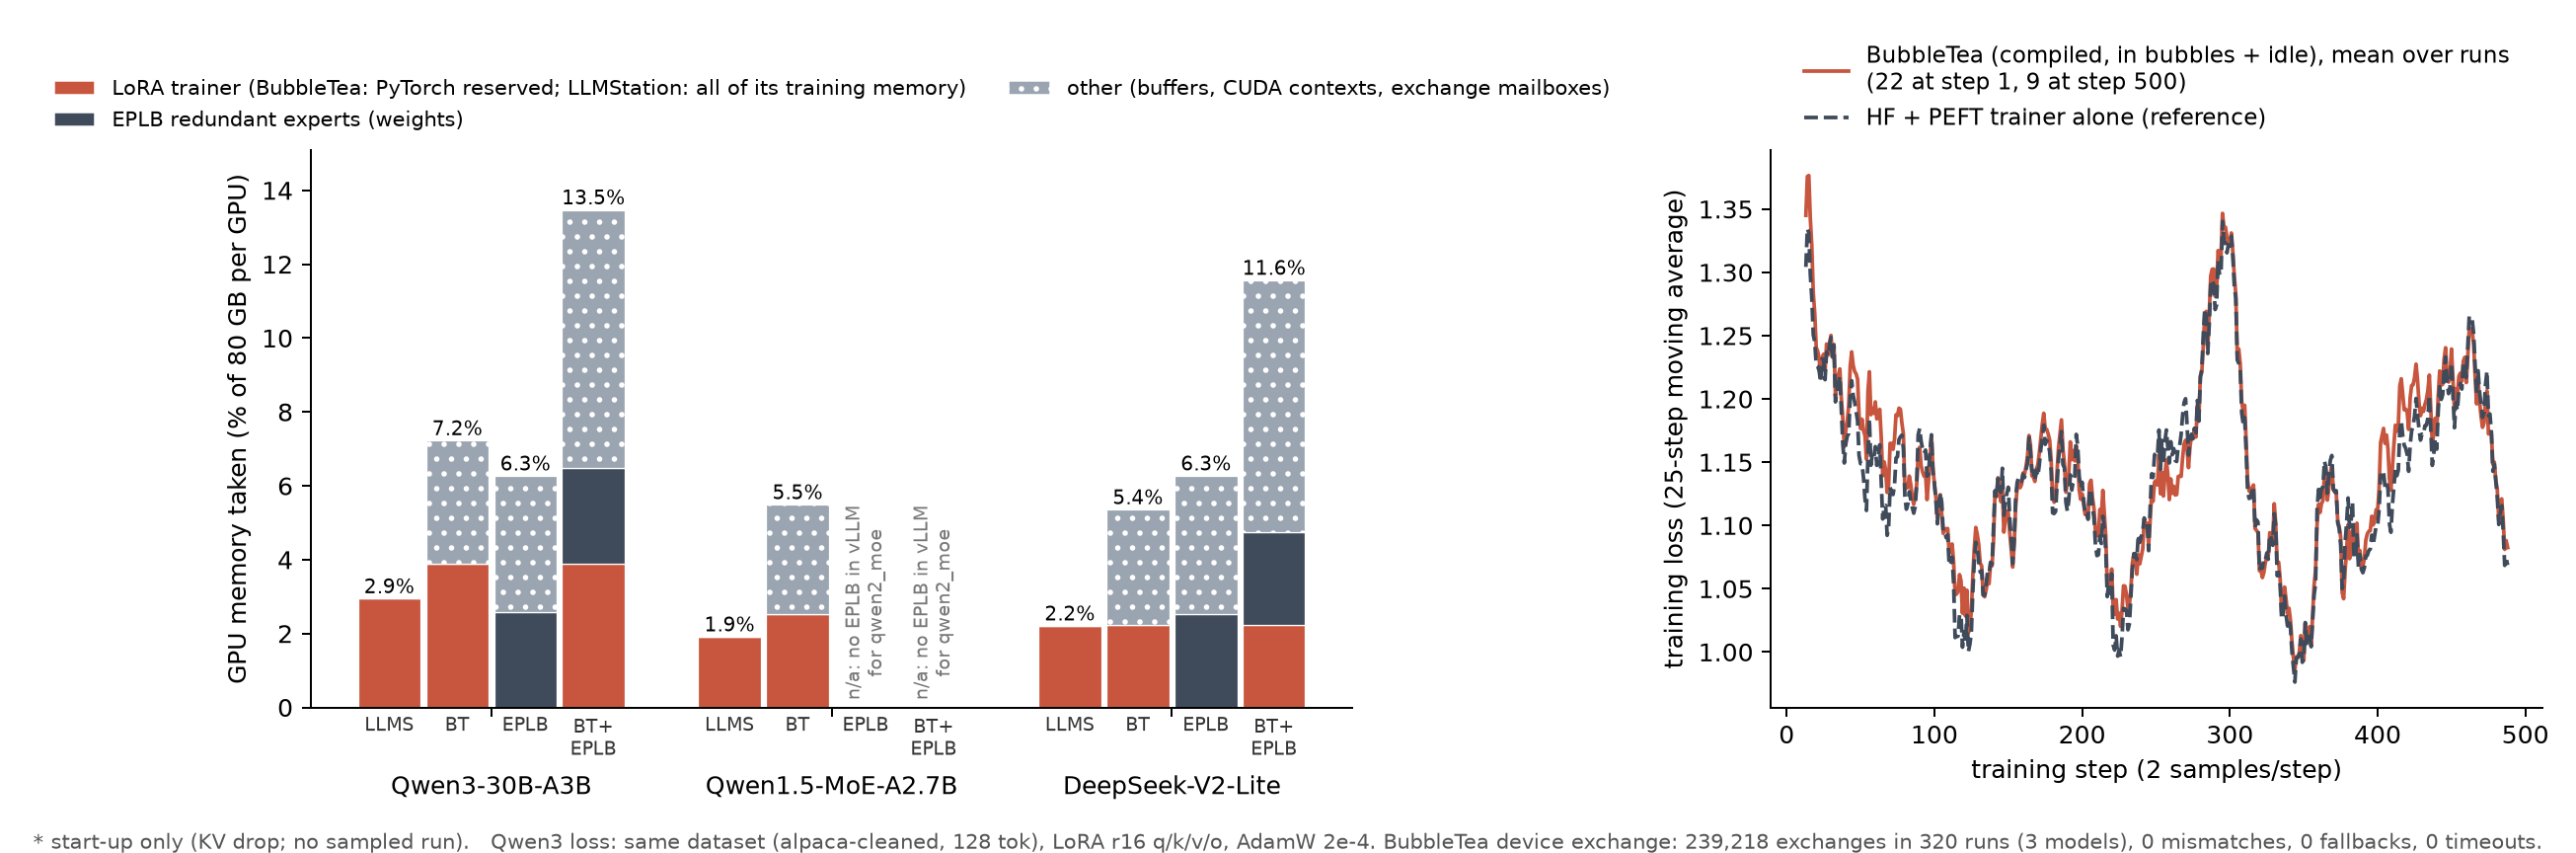
\includegraphics[width=0.66\textwidth]{eval/fig66_overheads.png}%
  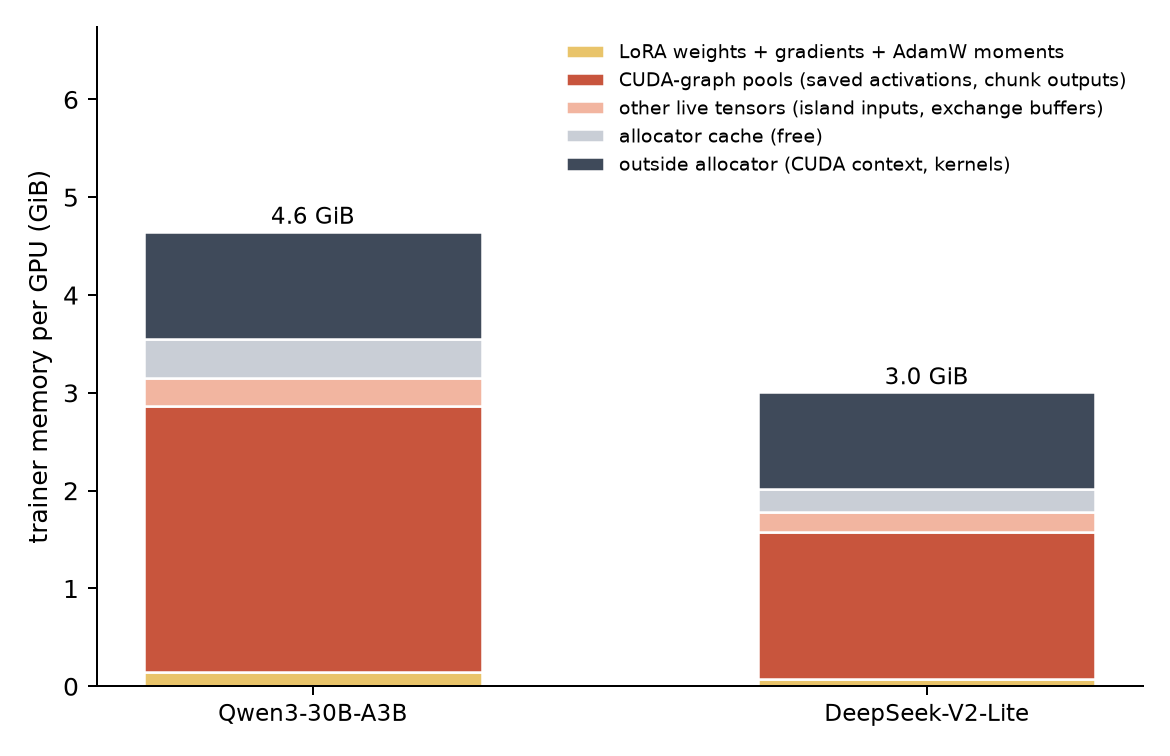
\includegraphics[width=0.33\textwidth]{eval/fig66_mem_breakdown.png}
  \caption{\textbf{Memory and correctness.} Left: GPU memory taken from
    serving by each system, with and without EPLB, and training loss of
    \sys{} against a stand-alone HF+PEFT trainer on the same data.
    Right: where the \sys{} trainer's memory goes, per GPU.}
  \label{fig:appx-eval-overheads}
\end{figure*}

\paragraph{Memory.}
Memory taken by the trainer is memory serving cannot use for its KV cache.
\sys{} takes 4.3--5.8\,GiB per GPU, 5--7\% of an 80\,GB A100
(Figure~\ref{fig:appx-eval-overheads}). LLMStation takes less, 1.5--2.4\,GiB,
because it trains inside the serving process and shares its CUDA context
and allocator.

The right panel of Figure~\ref{fig:appx-eval-overheads} shows where \sys{}'s
memory goes. The LoRA state itself, weights, gradients and AdamW moments, is
small: 0.14\,GiB per GPU on Qwen3-30B-A3B and 0.08\,GiB on DeepSeek-V2-Lite.
The largest item is the pool behind the compiled training graphs (2.7 and
1.5\,GiB), which holds the activations a step saves for its backward pass.
Next is the trainer's own CUDA context and kernels (about 1\,GiB), the
price of running it as a separate process. Neither grows with the serving
load or the prompt length. (We could not obtain the same breakdown for
Qwen1.5-MoE: the allocator instrumentation makes a known start-up race in
its serving kernels fire on every attempt.)

EPLB's redundant experts cost 5.0\,GiB per GPU on their own, and the two
together cost what their parts add up to: 10.8\,GiB on Qwen3-30B-A3B and
9.3\,GiB on DeepSeek-V2-Lite. vLLM does not support EPLB for Qwen1.5-MoE.

\paragraph{Correctness.}
\sys{} changes how a training step executes---it splits the step into
chunks, runs them in bubbles on two chains and exchanges activations
between GPUs through device-side mailboxes---but it must not change what the
step computes. We train Qwen3-30B-A3B with \sys{} and, separately, with a
stand-alone HF+PEFT trainer using the same data, LoRA configuration
and learning rate. The two loss curves track each other closely
(Figure~\ref{fig:appx-eval-overheads}): the 25-step moving averages differ by
1.2\% on average and by at most 4.5\% over 476 steps. Across 320 \sys{} runs,
the trainer performed 239{,}218 device-side exchanges with no
mismatch, fallback or timeout.
